\section{Point Estimation}

  Let's start with the most fundamental type of estimation. In point-estimation, we are interested in vector-valued estimates. We would like to construct an estimator $\delta$ that approximates the true parameter. 
  \begin{equation}
    \delta(\mathcal{D}) \approx \theta^\ast
  \end{equation} 

  \begin{definition}[Sampling Distribution]
    The probability distribution of the random variable $\delta(\mathcal{D})$ is called the \textbf{sampling distribution}. 
    \begin{enumerate}
      \item The standard deviation of $\delta(\mathcal{D})$ is the \textbf{standard error}. 
    \end{enumerate}
  \end{definition}

  The $\theta^\ast$ may be treated as fixed (in frequentist regime) or random (Bayesian). So we must determine what makes an approximation good or bad. Two such measures are 
  \begin{equation}
    \mathbb{P}( \|\theta^\ast - \delta(\mathcal{D}) \| < c)
  \end{equation} 
  or 
  \begin{equation}
    \mathbb{E} \big[ \| \theta^\ast - \delta(\mathcal{D}) \|^p \big]
  \end{equation} 

  We would like the sampling distribution of our statistic to give us good estimate in two ways. $\delta(\mathcal{D})$ should not be too far off from the actual parameter $\theta^\ast$ (bias is small), and $\delta(\mathcal{D})$ should not fluctuate too widely (variance of $\theta^\ast$ should be small). 

  \begin{definition}[Bias on an Estimator]
    The \textbf{bias} of an estimator is 
    \begin{equation}
      \mathrm{Bias}(\delta) = \big| \theta^\ast -\mathbb{E}_{\mathcal{D}}[\delta(\mathcal{D})] \big|
    \end{equation}
  \end{definition} 

  \begin{definition}[Variance of an Estimator]
    The \textbf{variance} of an estimator is 
    \begin{equation}
      \mathrm{Var}(\delta) = \mathbb{E} \big[ (\theta^\ast - \mathbb{E}_{\mathcal{D}}[\delta(\mathcal{D})])^2 \big]
    \end{equation}
  \end{definition}

\subsection{Common Estimators} 

  \begin{definition}[Sample Mean] 
    The \textbf{sample mean} is the estimator 
    \begin{equation}
      \delta(\mathcal{D}) = \frac{x_1 + \ldots + x_n}{n}
    \end{equation} 
    used to estimate the population mean.
  \end{definition}

  Note that this may or may not be a good estimator, depending on the distribution which we assume the $x_i$'s are coming from, whether they are independent, or other things.

  \begin{lemma}[Mean]
    The mean of $\overline{x}_n$ is $\mu$. 
    \begin{equation}
      \mu_{\overline{x}_n} = \mu
    \end{equation}
  \end{lemma}
  \begin{proof}
    \begin{equation}
      \mathbb{E}[\overline{x}_n] = \mathbb{E} \bigg[ \frac{1}{n} \sum_{i=1}^n x_i \bigg] = \frac{1}{n} \sum_{i=1}^n \mathbb{E}[x_i] = \mathbb{E}[x] = \mu
    \end{equation}
  \end{proof}

  \begin{lemma}[Variance]
    If the variance is finite and the samples are iid, then the variance of $\overline{x}_n$ is $\sigma^2 / n$, i.e. the standard error of $\overline{x}_n$ is $\sigma_{\overline{x}_n} = \sigma / \sqrt{n}$. 
    \begin{equation}
      \sigma_{\overline{x}_n} = \frac{\sigma}{\sqrt{n}}
    \end{equation}
    because 
    \begin{equation}
      \sigma^2_{\overline{x}_n} = \frac{1}{n^2} \sum_{i=1}^n \mathrm{Var}(x_i) = \frac{1}{n} \mathrm{Var}(x) = \frac{\sigma^2}{n}
    \end{equation}
     Practically, this tells us that when trying to estimate the value of a population mean, due to the factor of $1/\sqrt{n}$, reducing the error on the estimate by a factor of $2$ requires acquiring $4$ times as many observations in the sample. But realistically, the true standard deviation $\sigma$ is unknown, and so the standard error of the mean is usually estimated by replacing $\sigma$ with the sample standard deviation $S$ instead. 
    \begin{equation}
      \sigma_{\overline{x}_n} \approx \frac{S}{\sqrt{n}}
    \end{equation}
  \end{lemma}

  By CLT, $\overline{x}_n$ converges to $\mathcal{N}(\mu, \sigma^2/n)$ in distribution as $n \rightarrow +\infty$ (but in practicality, we assume this for $n \geq 30$). The fact that its mean and variance is $\mu$ and $\sigma^2 /n$ isn't that impressive. What is really impressive is that no matter what the distribution of $x$ is, the sampling distribution of the mean will be Gaussian. 

  \begin{example}[Sample Means]
    Here are some figures of sample means. Note that with a uniform parent distribution, the sampling distribution of its mean looks like a Gaussian even without a large $n$. However, this is not necessarily true for different parent distributions, such as the exponential. 
    \begin{figure}[H]
      \centering
      \begin{subfigure}[b]{0.48\textwidth}
      \centering
        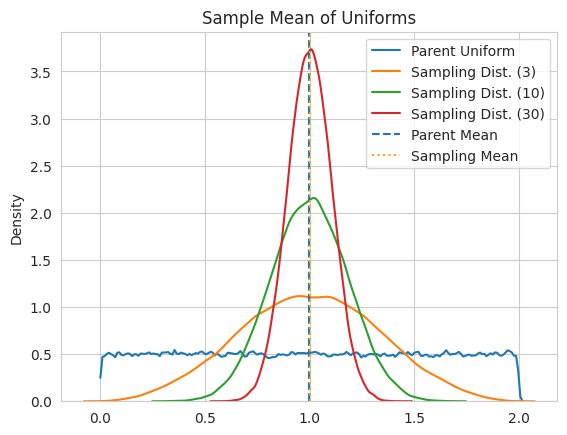
\includegraphics[width=\textwidth]{img/sample_mean_uniform.png}
        \caption{We plot the PDF of an $X \sim \mathrm{Uniform}[0, 2]$ random variable by taking 100k samples. We also take 100k samples from the sampling distribution of the mean $\overline{X}_{3}, \overline{X}_{10}, \overline{X}_{30}$. We can see that the standard deviation decreases by a factor of $\sqrt{n}$.}
        \label{fig:sample_mean_uniform}
      \end{subfigure}
      \hfill 
      \begin{subfigure}[b]{0.48\textwidth}
      \centering
        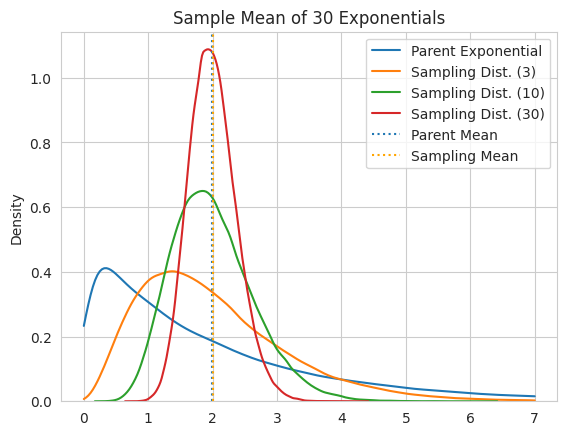
\includegraphics[width=\textwidth]{img/sample_mean_exp.png}
        \caption{We plot the PDF of an $X \sim \mathrm{Exponential}(1.5)$ random variable by taking 100k samples. We also take 100k samples from the sampling distribution of the mean $\overline{X}_{3}, \overline{X}_{10}, \overline{X}_{30}$. }
        \label{fig:sample_mean_exp}
      \end{subfigure}
      \caption{}
      \label{fig:sample_mean_examples}
    \end{figure}
  \end{example}

  If the parent distribution is normal, then we don't even need CLT to claim that the sampling distribution of the sample mean is normal, since sums of normals are normal. 

  Now the variance of the population is defined to be $\sigma^2 = \mathbb{E}[ (X - \mathbb{E}[X])^2 ]$, and by our rule of thumb, we can replace the expectations with sample means, by first setting $\mathbb{E}[X] = \widehat{\mu}$ and averaging out the values $(X - \widehat{\mu})^2$. 

  \begin{definition}[Sample Variance]
    Given a population $X$, our estimator for $\sigma^2 = \mathbb{E}[ (X - \mathbb{E}[X])^2 ]$ is simply the average of the squared distances of the $n$ samples $\{(x_i - \widehat{\mu})^2\}_{i=1}^n$. 
    \begin{equation}
      S^2_n = \widehat{\sigma}^2_n = \frac{1}{n} \sum_{i=1}^n ( x_i - \overline{x}_n)^2
    \end{equation}
    The mean and standard deviation of $S^2_n$ is denoted $\mu_{S^2_n}$ and $\sigma_{S^2_n}$. Note that there is a small difference that the sum for variance is divided by $n-1$ rather than $n$, since we want it to be unbiased, but we will correct this later. 
  \end{definition}

  While the CLT states that the sampling distribution of the sample mean will look approximately Gaussian, we do not have this luxury when looking at the sampling distribution of sample variance. 

  \begin{example}[Sample Variance]
    Take a look at the following sampling distributions of the sample variance. There does not seem to be strong signs of convergence to a Gaussian. Their means do not align either. 
    \begin{figure}[H]
      \centering
      \begin{subfigure}[b]{0.48\textwidth}
      \centering
        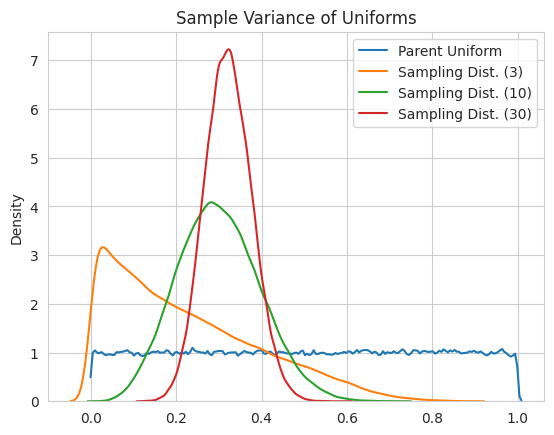
\includegraphics[width=\textwidth]{img/sample_variance_uniform.png}
        \caption{}
        \label{fig:sample_variance_uniform}
      \end{subfigure}
      \hfill 
      \begin{subfigure}[b]{0.48\textwidth}
      \centering
        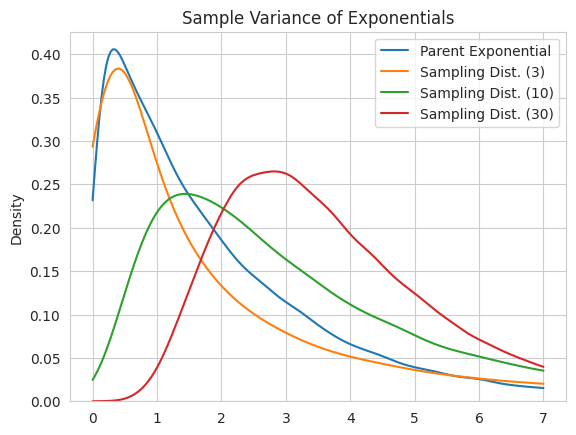
\includegraphics[width=\textwidth]{img/sample_variance_exp.png}
        \caption{}
        \label{fig:sample_variance_exp}
      \end{subfigure}
      \caption{}
      \label{fig:sample_variance_examples}
    \end{figure}
  \end{example}

\subsection{Sampling from Gaussians}

  Now if we assume that the parent distribution is Gaussian, then we can conclude some extra things and more kinds of distributions arise. Let $x_1, \ldots, x_n \sim \mathcal{N}(\mu, \sigma^2)$, with $\overline{x}_n$ the sample mean and $S^2_n$ the sample variance. Say that we want to find the distribution of $\overline{x}_n$. 
  \begin{enumerate}
    \item In the unrealistic case where we know the true $\sigma^2$, we don't even need to consider the sample variance. From the basic property of Gaussians, we know that $\overline{x}_n \sim \mathcal{N}(\mu, \sigma^2/n)$, or after standardizing, 
    \begin{equation}
      \frac{\overline{x}_n - \mu}{\sigma/\sqrt{n}} \sim \mathcal{N}(0, 1)
    \end{equation}
    \item In the realistic case where we don't know the true $\sigma^2$, we should replace it with our sample variance $S^2$, and it turns out that because of this extra uncertainty in the variance, our sampling distribution follows the student-t distribution, which can be interpreted as a mixture of Gaussians with differing variances. 
    \begin{equation}
      \frac{\overline{x}_n - \mu}{S/\sqrt{n}} \sim \mathrm{StudentT}(n-1)
    \end{equation}
  \end{enumerate}
  Now if we are interested in finding the distribution of $S^2_n$: 
  \begin{enumerate}
    \item In the unrealistic case where the know the true $\mu$, we don't need to consider the sampling distribution of $\overline{x}_n$. We have 
    \begin{equation}
      S^2_n = \frac{1}{n} \sum_{i=1}^n (x_i - \mu)^2 \sim \mathrm{Gamma}\Big( \frac{n}{2}, \frac{n}{2 \sigma^2} \Big)
    \end{equation}
    \item In the realistic case where we don't know $\mu$, we have 
    \begin{equation}
      \frac{n-1}{\sigma^2} S^2_n = \frac{1}{\sigma^2} \sum_{i=1}^n (x_i - \overline{x}_n )^2 \sim \chi^2 (n-1)
    \end{equation}
  \end{enumerate}

